\section{Parallelising Procedural GA using MPI}
\subsection{Parallel GA model}
The master-slave model of parallel GA is adopted for this implementation. The operation most commonly parallelised in master-slave model is the evaluation of the fitness function as in general this requires only individuals values not the entire population so that the communication is minimum between nodes. Parallelising the evaluation of fitness function is done by assigning a part of population to each node available in a cluster. Message passing occurs when slave nodes receive the subset of global population and returns evaluated fitness values to the master. 

Figure \ref{fig:flowchart_pga} represent the flowchart of implemented Parallel GA. Dotted line shows Message passing communication between Master and Slaves. This flowchart shows the diagram of implemented parallel GA using the procedural SGA discussed earlier in this section. As we can see from this diagram Master process responsible for initialising first generation of population, evaluate and report on them. The next task for the master process is to dividing up population among available slave processes. 

\begin{figure}[!hp]
    \vspace*{-1cm}
    \makebox[\linewidth]{
        \includegraphics[width=.9 \linewidth]{figs/flowchart_pga2.png}
    }
    \caption{Flowchart diagram of Implemented master-slave Parallel GA}
     \label{fig:flowchart_pga}
\end{figure}


The following subsections explain various MPI directives implemented.

\subsection{Initialising MPI environment}
As with all MPI program the message-passing environment needs to be initialised prior to calling any message-passing procedure. This is done by calling MPI\_Init() procedure on line 8 shown in the code fragments on Listing \ref{lst:pga_initialise_mpi}. MPI uses objects known as communicators and groups to define which collection of processes may communicate with each other. MPI\_Comm\_size() returns number of processes available for MPI communication and MPI\_Comm\_rank() returns its own unique rank id for identification within a communicator group.

\begin{lstlisting}[language=C, caption={Parallel GA implementation using MPI: Source code of main()}, label={lst:pga_initialise_mpi}]
MPI_Init(&argc, &argv);
MPI_Comm_size(MPI_COMM_WORLD, &numNodes); // How many nodes
MPI_Comm_rank(MPI_COMM_WORLD, &myId); // My Rank ID
\end{lstlisting}

\subsection{Creating MPI derived datatype for genotype}
MPI requires data to be in a contiguous memory location for marshalling and demarshalling of data to send and receive. Any non-primitive datatype needs to be defined for MPI to handle this properly. Listing \ref{lst:pga_mpi_create_struct} shows the procedure for creating a MPI derived datatype for the genotype struct of SGA. Line 14 contains the MPI routine MPI\_Type\_create\_struct() that requires 3 arrays containing information about user data types, their count and their offsets values within the struct along with original data type that is being converted and an MPI\_Datatype object where this routine will return the new type on success. In lines 7-12 the offsets values of genotype members are being stored in offsets array using C library macro offsetof() function.

\begin{lstlisting}[language=C, caption={Creating an MPI derived data type for genotype struct.}, label={lst:pga_mpi_create_struct}]
void create_mpi_genotype_struct(MPI_Datatype& mpi_genotype){
    const int nitems = 6;
    int blocklengths[6] = {NVARS, 1, NVARS, NVARS, 1, 1};
    MPI_Datatype types[6] = {MPI_DOUBLE, MPI_DOUBLE, MPI_DOUBLE, MPI_DOUBLE, MPI_DOUBLE, MPI_DOUBLE};
    
    MPI_Aint     offsets[6];
    offsets[0] = offsetof(genotype, gene);
    offsets[1] = offsetof(genotype, fitness);
    offsets[2] = offsetof(genotype, upper);
    offsets[3] = offsetof(genotype, lower);
    offsets[4] = offsetof(genotype, rfitness);
    offsets[5] = offsetof(genotype, cfitness);
    
    MPI_Type_create_struct(nitems, blocklengths, offsets, types, &mpi_genotype);
    MPI_Type_commit(&mpi_genotype);
}
\end{lstlisting}


\subsection{Partitioning of data}
Following strategy shown in Listing \ref{lst:pga_partitioning} is applied to partition the population among available nodes. A 2D array node\_data[][] shown in line 1 is used to hold the starting index and the row count for a given node id. From line 3 to line 11 the starting index and row counts are calculated and stored in node\_data[][] array for each node\_id. 

\begin{lstlisting}[language=C, caption={Partitioning population data among nodes}, label={lst:pga_partitioning}]
    int nodes_data[numNodes][2]; // Array to hold data partition information
    int start_i, num_rows;
    int chunk_size = (int)(ceil((double) POPSIZE / numNodes));
               
    for(int i = 0; i < numNodes; i++)
    {
        start_i = i * chunk_size;
        num_rows = min(chunk_size, POPSIZE - start_i);
        nodes_data[i][0] = start_i;
        nodes_data[i][1] = num_rows;
    }
\end{lstlisting}

\subsection{PGA v1}

\subsubsection{Master-Slave Communication}
In master-slave model all processes run the same MPI program. But depending on its role each process executes parts of the program. The parts of the main() shown in Listing \ref{lst:pga_mpi_main}. On line 3 each process gets its own communicator ID by calling MPI\_Comm\_rank(). Using this ID master process executes the master\_process() (line 5) and all other process executes slave\_process()(line 9). 

\begin{figure}[!htb]
        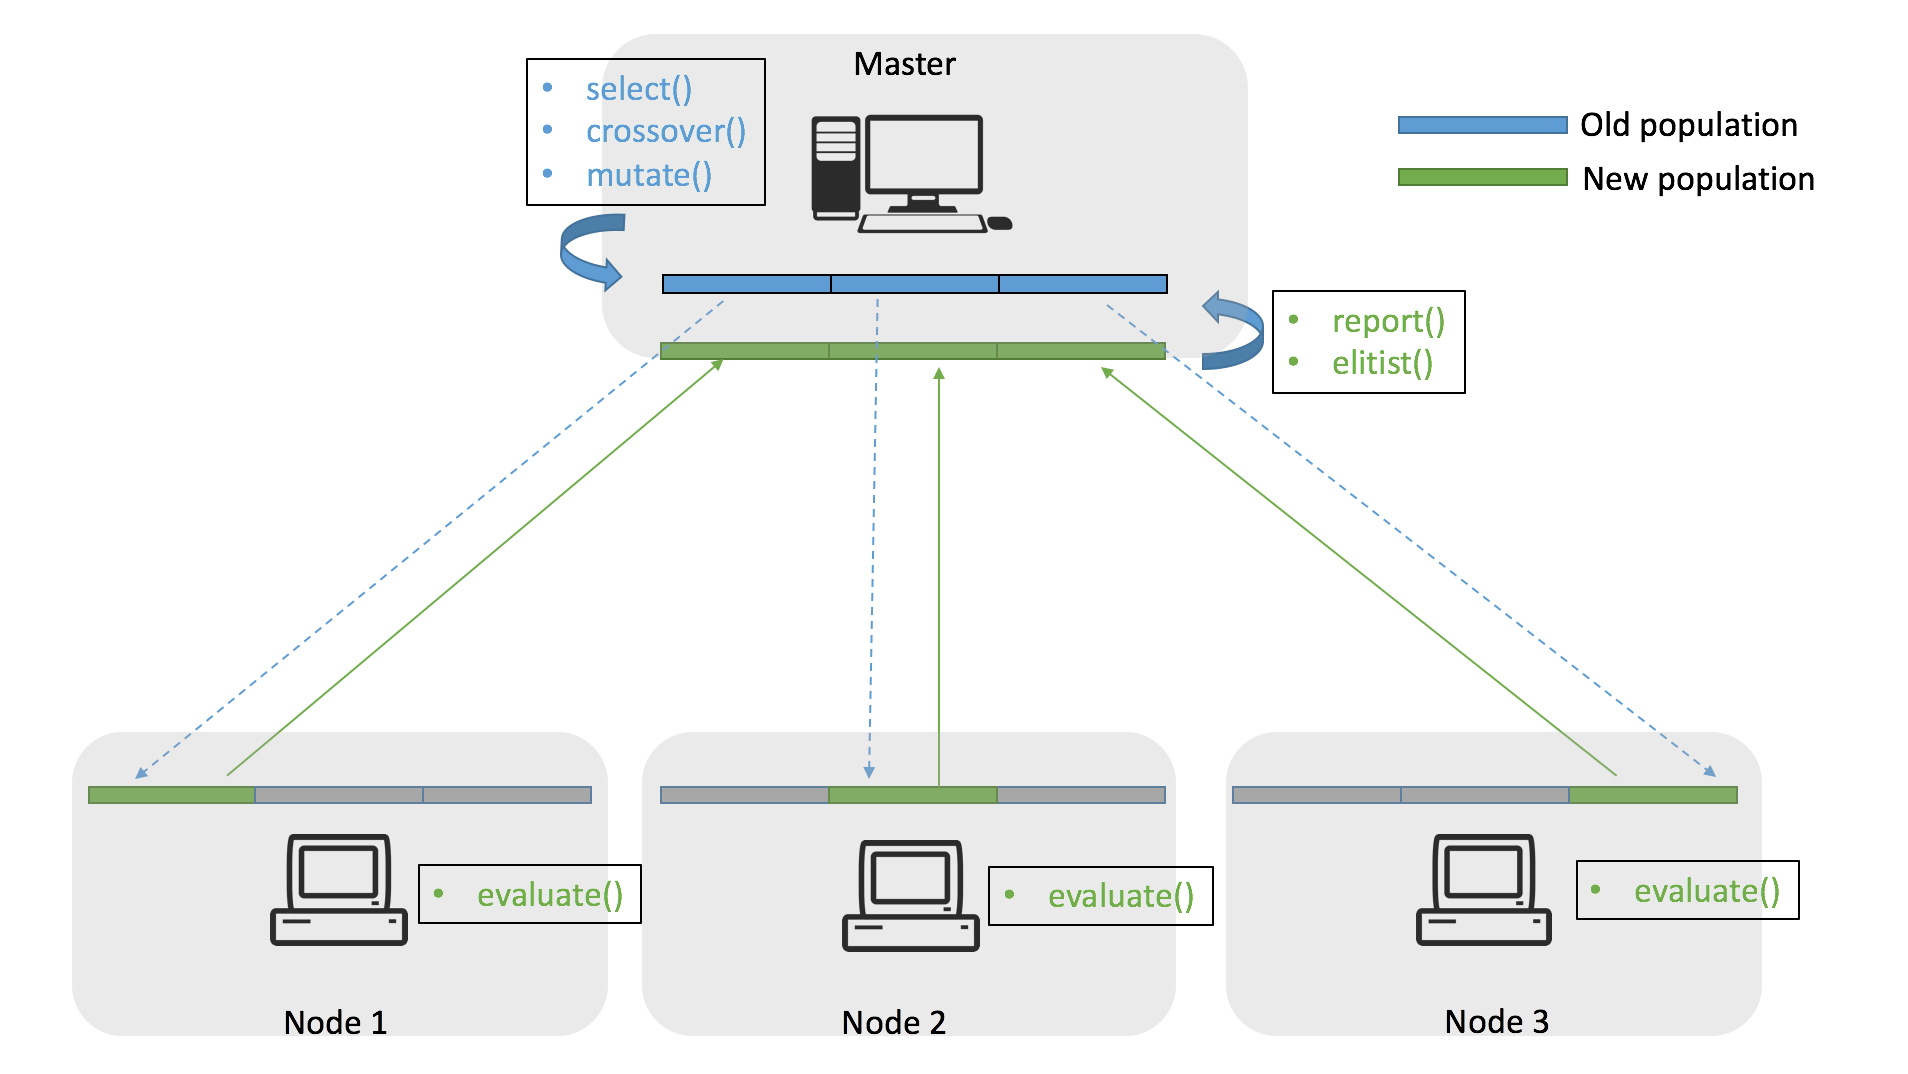
\includegraphics[width= \linewidth]{figs/pga_model_v1.png}
    \caption{PGA v1 model}
     \label{fig:pga_model_v1}
\end{figure}

For each generation, the master\_process() is responsible for performing selection, crossover and mutation operation on entire population ,  dividing population among all available nodes, updating all nodes with their parts of current population, collecting evaluated fitness values from each nodes, evaluate the best member for that generation, report and perform elitist operation on entire population. Where slave process is only responsible to receive a subset of population from master, evaluate their fitness values, send them back to master.  Figure \ref{fig:pga_model_v1} shows the master and slave data decomposition and the GA operation they perform on the population data depends on their role.

\begin{lstlisting}[language=C, caption={Master and slave pr}, label={lst:pga_mpi_main}]
ierr = MPI_Init(&argc, &argv);
ierr = MPI_Comm_size(MPI_COMM_WORLD, &numNodes); // How many nodes
ierr = MPI_Comm_rank(MPI_COMM_WORLD, &myId); // My Rank ID
    
if(myId == MASTER_ID) // Master Process
{
      master_process(filename, seed, mpi_genotype, nodes_data, start);
}
else // Slave processes
{  
    slave_process(seed, mpi_genotype, nodes_data);
}
\end{lstlisting}

\subsubsection{Master process}
In Listing \ref{lst:pga_master_process} parts of the master\_process() procedure is shown. After initialising the initial population master starts performing GA operation on them(lines 3-6). On lines 9-14 it starts sending subset of population to each nodes using MPI\_Send() routine. As we shall see in Listing \ref{lst:pga_slave_process} there is a corresponding MPI\_Recv routine call (line 2) invoked by the slave process. Master then evaluate it's own parts the population subset (line 17). On lines 20-25 master starts to gather the parts of population which have their fitness value calculated by the slave nodes. Then on line 27 master perform elitist() operation using entire population.

\begin{lstlisting}[language=C, caption={The master\_process() procedure.}, label={lst:pga_master_process}]
for(int generation = 0; generation < MAXGENS; generation++)
{   
      selector ( seed );
      crossover ( seed );
      mutate ( seed );     
      report(generation);

      int start_index, item_count;
      for(int nodeId = 1; nodeId < numNodes; nodeId++)
      {
          start_index = nodes_data[nodeId][0];
          item_count = nodes_data[nodeId][1];
          MPI_Send(&population[start_index], item_count, mpi_genotype, nodeId, SEND_DATA_TAG, MPI_COMM_WORLD);
        }
        
      /* Evaluate master's parts of the population */
      evaluate(nodes_data[0][0], nodes_data[0][1]);
        
      /* Collect all parts of new population from each node */
      for(int nodeId = 1; nodeId < numNodes; nodeId++)
      {
          start_index = nodes_data[nodeId][0];
          item_count = nodes_data[nodeId][1];
          MPI_Recv(&population[start_index], item_count, mpi_genotype, nodeId, RETN_DATA_TAG, MPI_COMM_WORLD, &status);
       }
                
      elitist();
}
\end{lstlisting}

\subsubsection{Slave process}
As we can see in Listing \ref{lst:pga_slave_process} the slave process starts with a MPI\_Recv() call on line 4. After receiving the parts for the population slave process perform evaluate() using its own starting index and row count on line 7. When the fitness evaluation is done it start to send the population part to master process by calling MPI\_Send() routine.


\begin{lstlisting}[language=C, caption={The slave\_process() procedure.}, label={lst:pga_slave_process}]
for(int generation = 0; generation < MAXGENS; generation++)
{
    /* Get a subset of population from master */
    ierr = MPI_Recv(&population[my_start], row_count, mpi_genotype, MASTER_ID, SEND_DATA_TAG, MPI_COMM_WORLD, &status);
        
    /* Perform fitness evaluation */
    evaluate (my_start, row_count);
        
    /* Send evaluated population to master */
    MPI_Send(&population[my_start], row_count, mpi_genotype, MASTER_ID, RETN_DATA_TAG, MPI_COMM_WORLD);
}
\end{lstlisting}


\subsection{PGA v2}
\subsubsection{Performance issue with PGA v1}
The first implementation of Master-slave GA as in PGA v1 distribute evaluation of fitness function among several slave processors while master executes the GA operations(selection, crossover and mutation). This implementation explore the search space in exactly same manner as a serial GA and follows exactly the same simple GA design guidelines. It is thought to be the case that, this implementation of master-slave parallel GA results in significant improvement in performance. However, as we shall see in Chapter \ref{empirical} when empirical studies were carried out the actual performance gains seemed to be worse than the serial GA. This is perhaps for the frequent MPI communication overhead that required in each generation for evaluating fitness values back and forth to the master and slave nodes. The execution time time of master-slave GAs have two components; the time used for communication between nodes and the time used in computation. So, the other reason is, master is responsible for performing all GA operations on entire population while slave nodes are mostly sitting idle during this time. With this approach slave nodes are under utilised where master node has a lot of workload 

So, in this version of PGA we tried to leverage some of the GA operations as well as evaluating fitness values to the slave nodes. The movements of population data and node specific GA operations are depicted in Figure \ref{fig:pga_model_v2}.

\begin{figure}[!htb]
        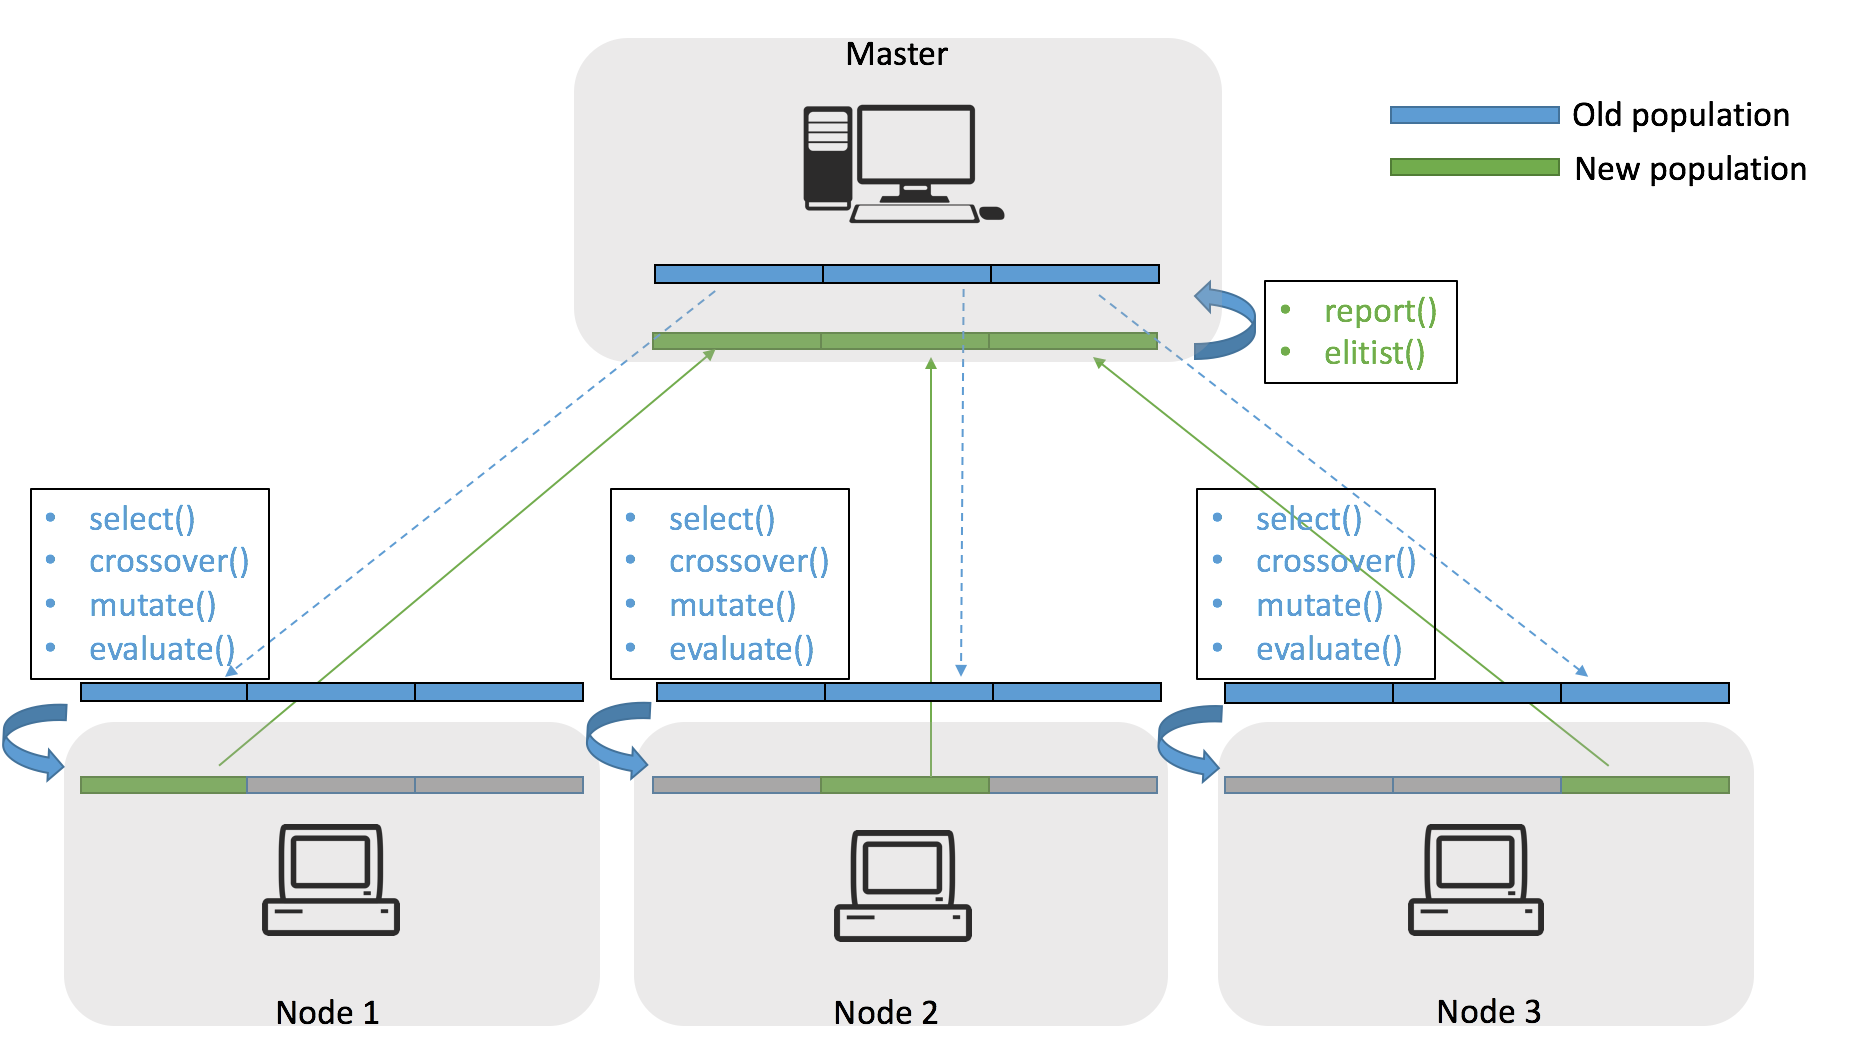
\includegraphics[width= \linewidth]{figs/pga_model_v2.png}
    \caption{PGA v2 model}
     \label{fig:pga_model_v2}
\end{figure}

\subsubsection{Using MPI Broadcast instead of explicit MPI Send/Recv}
To reduce communication overhead MPI collective routine \textbf{MPI\_Bcast()} is used by replacing  explicit \textbf{MPI\_Send() and MPI\_Recv()}. To ensure proper synchronisation among all nodes in the cluster the \textbf{MPI\_Barrier()} is called. When a process calls MPI\_Barrier(), it waits until all of the nodes also call this procedure.

Some part of this implementation is shown in Listing \ref{lst:pga_procedures}. On lines 5-9 master node initialises initial population and perform first elitist operation(keep\_the\_best( )). Slave nodes wait for these operation to complete because of MPI\_Barrier() call on line 12. On line 15 entire population is broadcasted with MPI\_Broadcast() call followed by another call to MPI\_Barrier().  On lines 20-21 all nodes determine their own data partition information. Then all nodes perform GA operations and evaluate the fitness values for the subpopulation(lines 22-27). On lines 32-36 each node then broadcasts its part of the population data. This followed by another synchronisation on line 38 before master node call the elitist() operation on entire population on line 43.

\begin{lstlisting}[language=C, caption={PGA v2 main() procedures.}, label={lst:pga_procedures}]
ierr = MPI_Comm_size(MPI_COMM_WORLD, &numNodes); // How many nodes
ierr = MPI_Comm_rank(MPI_COMM_WORLD, &myId); // My Rank ID
    
/* Initialise first gen population in master process */   
if(myId == MASTER_ID) // Master Process
{        
      initialize ( filename, seed );
      evaluate (0, POPSIZE );
      keep_the_best ( );
}

MPI_Barrier(MPI_COMM_WORLD);
   
/* Broadcast entire first generation from master process */
MPI_Bcast(population, POPSIZE + 1, mpi_genotype, MASTER_ID, MPI_COMM_WORLD);
   
MPI_Barrier(MPI_COMM_WORLD);
 
/* Each process does GA ops here on individual data parts */ 
int my_start = nodes_data[myId][0];
int row_count = nodes_data[myId][1];
for ( generation = 0; generation < MAXGENS; generation++ )
{      
     node_selector (my_start, row_count, seed );
     crossover ( seed );
     node_mutate ( my_start, row_count,seed );   
     evaluate (my_start, row_count);
         
       /* Sync message - 3 */
      MPI_Barrier(MPI_COMM_WORLD);
        
      for(int i = 0; i < numNodes; i++)
      {
          MPI_Bcast(&population[nodes_data[i][0]], nodes_data[i][1], mpi_genotype, i, MPI_COMM_WORLD);
          MPI_Barrier(MPI_COMM_WORLD);
      }
        
      MPI_Barrier(MPI_COMM_WORLD);
        
      if(myId == MASTER_ID) // Master Process
      {
          report(generation);
          elitist ( );
      }
        
      MPI_Barrier(MPI_COMM_WORLD);
}
\end{lstlisting}

\subsection{PGA v3}

\subsubsection{Running Time Analysis of node\_selector() Procedure}
\label{pga_runtime_analysis}
During empirical study of program running time, with PGA v2 we noticed some performance gain when number of processors are increased for smaller population size(5000). We also noticed there is a drop of speedup when population size is increased.

After a some investigation into this problem it was identified that the running time of \textbf{selector()} procedure is contributing for this unexpected result. The Listing \ref{lst:pga_select} parts of this procedure where we can see there is a nested for loop. The outer loop(line 2) on line has a range of \textit{$(0, n/p)$} and the inner loop(line 11) has a range of  \textit{$(0, p)$} where  \textit{n} is the population size and \textit{p} is number of processors. Thus this function has a running time complexity of $\mathcal{O}(n/p * n)$ which is essentially $\mathcal{O}(n^2)$.

Since, all nodes are executing this node\_selector() procedure using entire global population, the total running time is directly dependent upon the slowest node/processor in the cluster plus communication overheard for each generation cycles.


\begin{lstlisting}[language=C, caption={node\_select() procedure.}, label={lst:pga_select}]
/* Select survivors using cumulative fitness. */ 
for ( i = my_start; i < ends; i++ )
{ 
    p = r8_uniform_ab ( a, b, seed );
    if ( p < population[0].cfitness )
    {
        newpopulation[i] = population[0];   
    }
    else
    {
        for ( j = 0; j < POPSIZE; j++ )
        {
            if ( population[j].cfitness <= p && p < population[j+1].cfitness )
            {
                newpopulation[i] = population[j+1];
            }
        }
    }
}
\end{lstlisting}


\subsubsection{Limiting Selection to Partial Population}
Based on the analysis discussed above, in this implementation the \textbf{selector()} procedure is modified so that the selection is done using nodes local subpopulation. Thus this would result in running time complexity of $\mathcal{O}((n/p) * (n/p))$ i.e . $\mathcal{O}((n/p)^2)$ Theoretically, if we could add more nodes i.e. processors we could reduce the affect of population size increases for this procedure proportionally. We know that number of processor cannot always be matched with population size increases but for a reasonably large population size (not infinite), adding in extra nodes can reduce the running time complexity of this function significantly. Figure \ref{fig:pga_model_v3} shows the data partition and GA operation for master and slave nodes. All GA operation including selection is done on subpopulation.

\begin{figure}[!htb]
        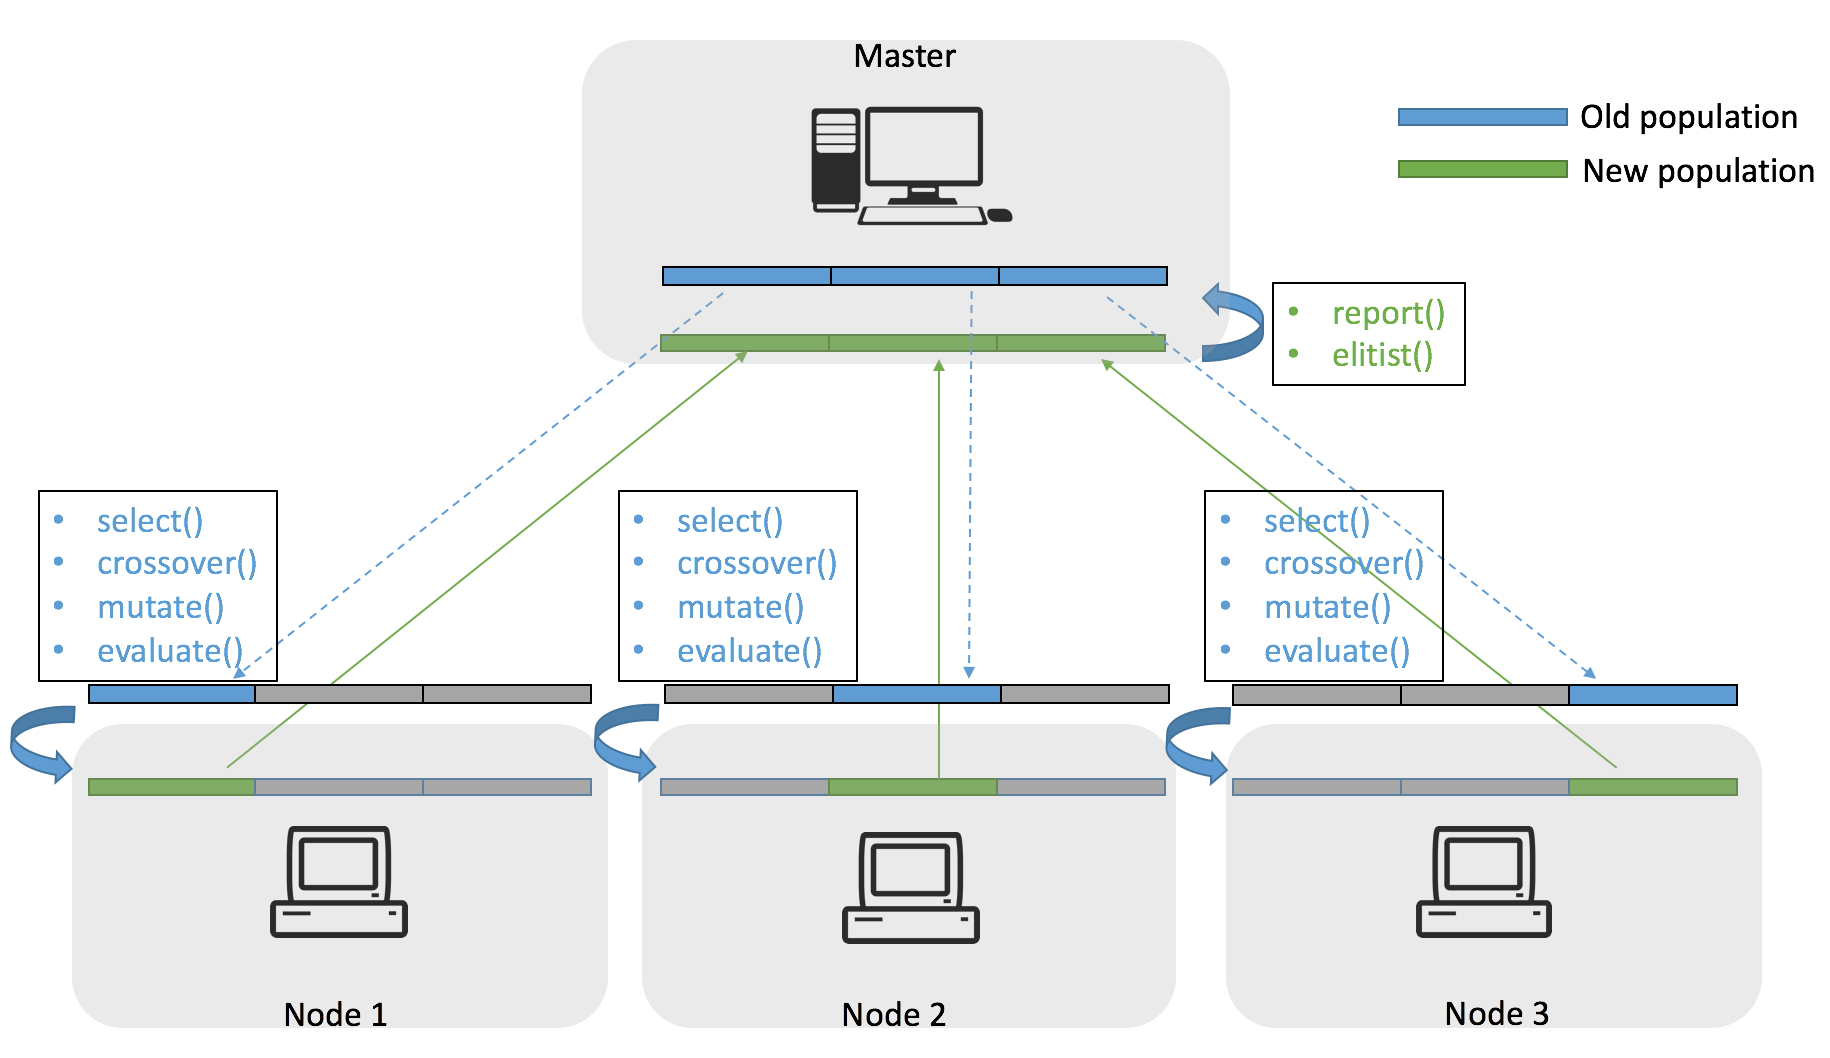
\includegraphics[width= \linewidth]{figs/pga_model_v3.png}
    \caption{PGA v3 model}
     \label{fig:pga_model_v3}
\end{figure}

Changes to the selector functions are shown in Listing \ref{lst:pga_select_changes} where the range inner for loop at line 10 is limited for the local subpopulation only which gives a range of \textit{$(0, n/p)$}.

\begin{lstlisting}[language=C, caption={Changes made in node\_select() procedures.}, label={lst:pga_select_changes}]
for ( i = my_start; i < ends; i++ )
{ 
    p = r8_uniform_ab ( a, b, seed );
    if ( p < population[my_start].cfitness )
    {
        newpopulation[i] = population[my_start];      
    }
    else
    {
        for ( j = my_start; j < ends; j++ )
        { 
            if ( population[j].cfitness <= p && p < population[j+1].cfitness )
            {
                newpopulation[i] = population[j+1];
            }
        }
    }
}
\end{lstlisting}

\subsection{Issues with Serialising Dynamic Data}
The SGA implementation allows population size, number of variables in a chromosome and number of generation can only be modified at compile time. To carry out the experiments we needed the PGA accept these parameters at runtime. So, an attempt was made to change these parameters at runtime with command line arguments. After a week of trials, this attempt was unsuccessful because of a number of reasons which are discussed here. Part of the problem was due to the data structure chosen to represent the chromosome which contains three static array members. The length of these arrays are defined at compile time. Population are initialised inside initialize\(\) procedure (Listing \ref{lst:initialize_proc}). Each individual is initialised with random permissible value. In this trial changes were made to the genotype data structure so that it could be initialised with dynamic arrays using malloc(). Program was compiled normally without any error. But during testing the PGA failed to produce acceptable outcome.

To find the underlying issue GDB was used to debug the problem. During this debugging program was run with a population size of 5. So the best member of a generation is kept  at index 5.
 
It was noticed(GDB output - Listing \ref{lst:gdb_output}) that some values of population members were changing unexpectedly. As we can see from the source code given in Appendix \ref{src:sga_proc.cpp} the initialize() procedure only assign initial value for \textbf{lbound}, \textbf{ubound} and \textbf{gene}. In this debugging session, the values of i, j and the best individual(population[5]) was monitored to catch unexpected any change. On line 42 we see that the value of  population[5].gene is 0x626330. But on next step on line 54 this value has changed to 0x3fe197d48c1f329c. We know that the initialize() procedure only assign values for the population member from 0 to (POPSIZE - 1) which is 4 in this run. So, the changes in population[5] is unexpected. It appeared that even though no value was assigned for best individual (which is population[5]), its member's values were changing. After looking more closely, it was noticed that the value that was being assigned to a data member for one individual was appearing inside some other individual's data member. Which means values were being assigned into wrong memory location. This indicated that malloc() for initialising the population array was not correct.


\begin{lstlisting}[style=BashInputStyle, label={lst:gdb_output}]
847 population[j].gene[i] = r8_uniform_ab ( lbound, ubound, seed );
1: population[5] = {fitness = 0, rfitness = 1.6304166312761136e-322, 
_ cfitness = 0, gene = 0x626330}
2: i = 0
3: j = 2
(gdb) 
840 for ( j = 0; j < POPSIZE; j++ )
1: population[5] = {fitness = 0, rfitness = 1.6304166312761136e-322, 
_ cfitness = 4.147546169663503, gene = 0x626330}
2: i = 0
3: j = 2
(gdb) 

.....

840 for ( j = 0; j < POPSIZE; j++ )
1: population[5] = {fitness = 0, rfitness = 1.6304166312761136e-322, 
_ cfitness = 4.147546169663503, gene = 0x626330}
2: i = 1
3: j = 1
(gdb) 
842 population[j].fitness = 0;
1: population[5] = {fitness = 0, rfitness = 1.6304166312761136e-322, 
_ cfitness = 4.147546169663503, gene = 0x626330}
2: i = 1
3: j = 2
(gdb) 
843 population[j].rfitness = 0;
1: population[5] = {fitness = 0, rfitness = 1.6304166312761136e-322, 
_ cfitness = 4.147546169663503, gene = 0x626330}
2: i = 1
3: j = 2
(gdb) 
844 population[j].cfitness = 0;
1: population[5] = {fitness = 0, rfitness = 1.6304166312761136e-322, 
_ cfitness = 4.147546169663503, gene = 0x626330}
2: i = 1
3: j = 2
(gdb) 
847 population[j].gene[i] = r8_uniform_ab ( lbound, ubound, seed );
1: population[5] = {fitness = 0, rfitness = 1.6304166312761136e-322, 
_ cfitness = 4.147546169663503, gene = 0x626330}
2: i = 1
3: j = 2
(gdb) 
840 for ( j = 0; j < POPSIZE; j++ )
1: population[5] = {fitness = 0, rfitness = 1.6304166312761136e-322, 
_ cfitness = 4.147546169663503, gene = 0x3fe197d48c1f329c}
2: i = 1
3: j = 2
(gdb) 
842 population[j].fitness = 0;
1: population[5] = {fitness = 0, rfitness = 1.6304166312761136e-322, 
_ cfitness = 4.147546169663503, gene = 0x3fe197d48c1f329c}
2: i = 1
3: j = 3
\end{lstlisting}

After this discovery, one and half week time was spent on how to allocate memory correctly for the \textbf{genotype} struct. But it seemed quite complicated to do so with three variable length array members in a struct. By researching on Internet about this, it was found that this issue is known as Variable Length Array In Struct(VLAIS). And with further research, some discussions related to this topic was found in Stackoverflow. The suggestions there were indicating that VLAIS is permissible on specific compiler i.e GCC C99 compatible only.  In one discussion posted on Stackoverflow \footnote{http://stackoverflow.com/questions/21804994/using-a-struct-member-as-array-size-in-the-same-struct} related to this topic further suggested that that variable-length arrays in structs is permissible in gcc (and the newest C-standards), but the variable array must always be the last member of the struct (so the compiler knows where all members are). In particular this means:

\begin{enumerate}
	\item There can be only one variable-length array
	\item If the struct is a member of another struct, it has to be the last member of that struct.
\end{enumerate}

Another post \footnote{http://stackoverflow.com/questions/17552312/multiple-flexible-array-in-a-struct-in-c} also suggested that it is not possible to have more than one flexible-array member in a struct.

There is no clear information whether mpic++ compiler has support for this feature of gcc too or not. The alternative solution to this problem would be to replace struct data structure with combination of C++ objects and vectors. Since this would have involved making a considerable changes to actual SGA implementation and possibilities of going back to the earlier problem with Object-oriented GA, a decision was made to leave these parameters to be defined at compile time.
